% SVN info for this file
\svnidlong
{$HeadURL$}
{$LastChangedDate$}
{$LastChangedRevision$}
{$LastChangedBy$}

\chapter{Spazi topologici}
\labelChapter{spazitopologici}

\begin{introduction}
‘‘La Topologia generale è una malattia da cui l'umanità guarirà presto.''
\begin{flushright}
	\textsc{Henri Poincaré,} dopo aver letto le prime pagine di un libro di Topologia.
\end{flushright}
\end{introduction}
\lettrine[findent=1pt, nindent=0pt]{I}{mmaginiamo} di avere un oggetto costituito di un magico \emph{materiale elastico} che possiamo allungare, piegare, torcere e rimpicciolire a piacere, ma che non possiamo né strappare né incollarne parti. L'oggetto che otteniamo dopo queste deformazioni lo consideriamo ‘‘equivalente'' a quello iniziale. Che proprietà si mantengono prima e dopo?\\
Il principale scopo della \textit{Topologia} è studiare proprio le proprietà che rimangono invariate da queste deformazioni continue. Per far ciò, è necessario dotare un insieme di una struttura, detta \textbf{topologia}, che permetta la definizione di \textbf{continuità} di una funzione e di \emph{omeomorfismo}, generalizzando così quello che abbiamo chiamato ‘‘deformazioni''.\\
In questo capitolo ci occuperemo dunque di introdurre questi concetti fondamentali per poi studiare alcuni risultati che ne conseguono. Inoltre, affronteremo alcuni degli \emph{assiomi di separazione} e la nozione di \emph{distanza}.
\section{Spazio topologico}
\begin{define}[Spazio topologico e assiomi degli aperti.]~{}\\
	Uno \textbf{spazio topologico}\index{spazio!topologico} $\left(X, \topo\right)$ è un insieme $X$ con una famiglia di sottoinsiemi $\topo\subseteq\setpart{X}$ detta \textbf{topologia}\index{topologia} che soddisfano i seguenti assiomi (detti \textbf{assiomi degli aperti}\index{assiomi topologici!degli aperti}):
	\begin{enumerate}
		\item \textit{Il vuoto e l'insieme stesso sono aperti della topologia}: $\emptyset,\ X\in\topo$ .
		\item \textit{L'unione arbitraria di aperti è un aperto}: dati $\left\{A_i\right\}_{i\in I}$ tali che $A_i\in\topo,\ \forall i\in I$ ($\left| I\right|\leq \infty$), allora $\displaystyle\bigcup_{i\in I}A_i=A\in\topo$ .
		\item \textit{L'intersezione finita di aperti è aperta}: dati $\left\{A_i\right\}_{i\in I}$ tali che $A_i\in\topo,\ \forall i\in I$ ($\left|I\right|< \infty$), allora $\displaystyle\bigcap_{i\in I}A_i=A\in\topo$.
	\end{enumerate}
	Gli elementi di $\topo$ si dicono \textbf{aperti}\index{aperto} della topologia.
\end{define}

\begin{define}[Spazio topologico e assiomi dei chiusi.]~{}\\
 Si può definire equivalentemente su X una topologia $\topo$ usando gli \textbf{assiomi dei chiusi}\index{assiomi topologici!dei chiusi}:
	\begin{enumerate}
		\item \textit{Il vuoto e l'insieme stesso sono chiusi della topologia}: $\emptyset,\ X\in\topo$.
		\item \textit{L'unione finita di chiusi è un chiuso}: dati $\left\{C_i\right\}_{i\in I}$ tale che $C_i\in\topo,\ \forall i\in I$ ($\left|I\right|< \infty$), allora $\displaystyle\bigcup_{i\in I}C_i=C\in\topo$ .
		\item \textit{L'intersezione arbitraria di chiusi è un chiuso}: dati $\left\{C_i\right\}_{i\in I}$ tale che $C_i\in\topo,\ \forall i\in I$ ($\left|I\right|\leq \infty$), allora $\displaystyle\bigcap_{i\in I}C_i=C\in\topo$.
	\end{enumerate}
	Gli elementi di $\topo$ si dicono \textbf{chiusi}\index{chiuso} della topologia.
\end{define}

\begin{observe}
	Per verificare il terzo assioma degli aperti (o, equivalentemente, il secondo dei chiusi) è sufficiente verificare che sia vero per \textit{soli due sottoinsiemi} qualunque, in quanto poi è verificato per induzione.
\end{observe}

\begin{examples}~{}
	\begin{itemize}
		\item \textbf{Topologia discreta}\index{topologia!discreta}: $\topo=\setpart{X}$, \textit{tutti} gli insiemi sono \textit{aperti}.
		\item \textbf{Topologia banale}\index{topologia!banale}: $\topo=\{\emptyset,\ X\}$, gli \textit{unici} aperti sono \textit{banali}.
	\end{itemize}
\vspace{-3mm}
\end{examples}
\subsection{Distanza e spazi metrici}
\begin{define}[Distanza.]~{}\\
	Su un insieme $X$ una funzione $\funz{d}{X\times X}{\realset}$ è una \textbf{distanza}\index{distanza} se:
	\begin{enumerate}
		\item \textbf{Positività della distanza}: $\forall x,\ y\in X\quad \mvf{d}{x}{y}\geq 0$ e $\mvf{d}{x}{y}=0\iff x=y$.
		\item \textbf{Simmetria}: $\forall x,\ y\in X\quad \mvf{d}{x}{y}=\mvf{d}{y}{x}$.
		\item \textbf{Disuguaglianza triangolare}\index{disuguaglianza triangolare}: $\forall x,\ y,\ z\in X\quad \mvf{d}{x}{z}\leq\mvf{d}{x}{y}+\mvf{d}{y}{z}$.
	\end{enumerate}
\vspace{-3mm}
\end{define}
\begin{define}[Spazio metrico.]~{}\\
	Uno \textbf{spazio metrico}\index{spazio!metrico} $\left(X, d\right)$ è un insieme su cui è definita una distanza.
\end{define}
\begin{define}[Palla aperta e topologia indotta dalla distanza.]~{}\\
	Definita la \textbf{palla aperta di centro}\index{palla aperta} $x$ come l'insieme degli elementi di $X$ che soddisfano la seguente condizione:
	\begin{equation}
		B_{\epsilon}\left(x\right)=\left\{y\in X\mid \mvf{d}{x}{y}<\epsilon\right\}
	\end{equation}
	Ogni spazio metrico ha una \textbf{topologia} $\topo_d$ \textbf{indotta dalla distanza}, i cui aperti sono definiti come:
	\begin{equation}
		A\subseteq X \text{ aperto } \left(A\in\topo\right) \text{ se } \forall x\in A,\ \exists \epsilon>0\ \colon B_{\epsilon}\left(x\right)\subseteq A.
	\end{equation}
\vspace{-6mm}
\end{define}
\begin{examples}~{}
	\begin{itemize}
		\item Su un qualunque insieme $X$ si può definire la \textit{distanza banale}:
		\begin{equation}
			\mvf{d}{x}{y}=\begin{cases} 
				0 & \text{se }x=y\\
				1 & \text{se }x\neq y
			\end{cases}
		\end{equation}
		In questo modo, ogni punto è una palla aperta e dunque ogni sottoinsieme è un aperto, dando allo spazio la \textit{topologia discreta}. In particolare, ogni insieme può essere uno spazio metrico.
		\item Su $X=\realset$ si può definire come distanza il \textit{valore assoluto} $\mvf{d}{x}{y}=\left|x-y\right|$, che induce la \textbf{topologia Euclidea}\index{topologia!Euclidea} $\eucl$, definita con le palle aperte di raggio $\epsilon$:
		\begin{equation}
			B_{\epsilon}\left(x\right)=\left\{y\in \realset\mid \left|x-y\right|<\epsilon\right\}
		\end{equation}
		Nel seguente modo:
		\begin{equation*}
			A\subseteq \realset \text{ aperto } \left(A\in\eucl\right) \text{ se } \forall x\in A,\ \exists \epsilon>0\ \colon B_{\epsilon}\left(x\right)\subseteq A.
		\end{equation*}
		\item Su $X=\realset^n$ si può definire come distanza la \textit{norma Euclidea}: $\mvf{d}{x}{y}=\labs x-y\rabs$ che induce la \textit{topologia Euclidea} $\eucl$ in modo analogo al caso precedente.
		\begin{gather*}
			B_{\epsilon}\left(x\right)=\left\{y\in \realset^n\mid \labs x-y\rabs<\epsilon\right\}\\
			A\subseteq \realset^n \text{ aperto } \left(A\in\eucl\right) \text{ se } \forall x\in A,\ \exists \epsilon>0\ \colon B_{\epsilon}\left(x\right)\subseteq A.
		\end{gather*}
	\end{itemize}
\vspace{-6mm}
\end{examples}
\begin{attention}
	Non tutte le topologie sono indotte da una distanza! Se esiste una palla $B_\epsilon\left(x\right)$ che \textit{non} è aperta per qualunque distanza $d$, allora la topologia non è indotta da una metrica. Ad esempio, definiamo la \textbf{topologia dei complementari finiti} o \textbf{topologia cofinita}\index{topologia!cofinita} sull'insieme $X$ nel modo seguente:
	\begin{equation*}
		A\subseteq X \text{ aperto } \left(A\in CF\right) \text{ se }  X\setminus A \text{ è finito.}\qquad
		C\subseteq X \text{ chiuso } \left(C\in CF\right) \text{ se }  C \text{ è finito.}
	\end{equation*}
	\begin{itemize}
		\item Se un aperto $A$ è tale se il suo complementare $\mathcal{C}A$ è finito, si ha che:
		\begin{equation}
			A=\mathcal{C}\left(\mathcal{C}A\right)=X\setminus\left(X\setminus A\right)=X\setminus\left\{\text{un numero finito di punti}\right\}
		\end{equation}
		In altre parole $A$ aperto equivale ad $X$ privato al più di un numero finito di punti.
		\item Se $X$ è finito, la topologia $CF$ coincide con la topologia discreta: ogni sottoinsieme di $X$ è finito e dunque un aperto.
		\item Se $X$ è infinito, ad esempio $\realset$, la topologia \textit{non} è quella discreta: $[0,\ 1]$ per la topologia discreta è un chiuso ma per quella $CF$ non lo è in quanto \textit{non} è finito.
	\end{itemize}
Sia $X$ infinito con topologia cofinita e supponiamo per assurdo che essa sia indotta da una metrica $d$. Consideriamo $x,\ y\in X$ distinti e definiamo $\epsilon \coloneqq \mvf{d}{x}{y} >0$.\\
Prendiamo le palle aperte $U=B_{\epsilon/2}\left(x\right)$ e $V=B_{\epsilon/2}\left(y\right)$: esse per \textit{disuguaglianza triangolare} hanno intersezione aperta e vuota $U\cap V=\emptyset$. Tuttavia, essendo degli aperti devono essere della forma $U=X\setminus \{\text{un numero finito di punti}\}$ e $V=X\setminus \{\text{un numero finito di punti}\}$, dunque l'intersezione è non vuota. Ma allora abbiamo un assurdo: $U\cap V$ risulta essere contemporaneamente vuoto e non vuoto. La cofinita pertanto \textit{non} è dunque una topologia indotta da una metrica.
\end{attention}
\subsubsection{Norme esotiche}
Possiamo definire su $\realset^n$ una famiglia di distanze dette \textbf{norme}\index{norma}; qui di seguito ne elenchiamo alcune. Definiti i punti $x=\left(x_1,\ldots, x_n\right),\ y=\left(y_1,\ldots, y_n\right)\in\realset^n$ abbiamo:
\begin{multicols}{2}
	\begin{itemize}
	\item \textbf{Norma infinito}:
	\[\mvf{d_\infty}{x}{y}=\max_{i}{\left|x_i-y_i\right|}\]
	\item \textbf{Norma uno}:
	\[\mvf{d_1}{x}{y}=\sum_{i=1}^{n}\left|x_i-y_i\right|\]
\end{itemize}
\begin{itemize}
	\item \textbf{Norma due}:
	\[\mvf{d_2}{x}{y}=\sqrt{\sum_{i=1}^{n}\left|x_i-y_i\right|^2}\]
	\item \textbf{Norma p}:
	\[\mvf{d_p}{x}{y}=\sqrt[\leftroot{1}\uproot{3}p]{\sum_{i=1}^{n}\left|x_i-y_i\right|^p}\]
\end{itemize}
\end{multicols}
\noindent Si ha $\displaystyle \lim_{p \to +\infty}d_p=d_\infty$. Valgono inoltre le seguenti disuguaglianze:
\begin{equation}
\forall x,\ y\in\realset^n\quad \mvf{d_\infty}{x}{y}\leq\mvf{d_2}{x}{y}\leq\mvf{d_1}{x}{y}\leq n\mvf{d_\infty}{x}{y}
\end{equation}
\vspace{-6mm}
\begin{demonstration}
Supponiamo senza perdere di generalità che $\mvf{d_\infty}{x}{y}=\left|x_1-y_1\right|$.
\begin{gather*}
\mvf{d_2}{x}{y}=\sqrt{\left|x_1-y_1\right|^2+\ldots+\left|x_n-y_n\right|^2}\geq\sqrt{\left|x_1-y_1\right|^2}=\left|x_1-y_1\right|=\mvf{d_\infty}{x}{y}\\
\mvf{d_2}{x}{y}=\left|x_1-y_1\right|+\ldots+\left|x_n-y_n\right|\leq\left|x_1-y_1\right|+\ldots+\left|x_1-y_1\right|=n\left|x_1-y_1\right|=n\mvf{d_\infty}{x}{y}
\end{gather*}
Notiamo che $\left|x_i-y_i\right|$ sono sempre positive, allora sia $a_i\coloneqq\left|x_i-y_i\right|$. Segue che $a_1^2+\ldots+a_n^2\leq (a_1+\ldots+a_n)^2$ perché $a_i,\ldots,a_n\geq0$. Allora:
\begin{equation*}
\sqrt{a_1^2+\ldots+a_n^2}\leq a_1+\ldots+a_n\implies d_2\leq d_1
\end{equation*}
\vspace{-6mm}
\end{demonstration}
Queste disuguaglianze danno le seguenti inclusioni\footnote{Qui $B_i\left(r\right)$ indica la palla aperta di raggio $r$ e centro fissato $x$ rispetto alla norma $i$.}:
\begin{equation}
B_1\left(\epsilon\right)\subseteq B_2\left(\epsilon\right)\subseteq B_\infty\left(\epsilon\right)\subseteq B_1\left(n\epsilon\right)
\end{equation}
\begin{center}
	\hspace*{-12cm}\begin{minipage}{.2\linewidth}
		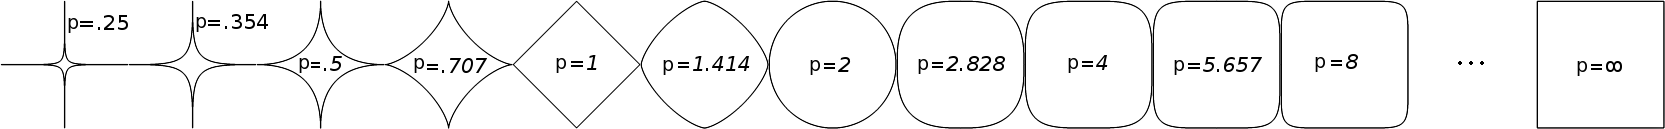
\includegraphics[trim=18.1cm 0cm 0cm 0cm,clip,scale=0.37]{images/pnorm.png}
	\end{minipage}
\end{center}
Questo ci porta a dire che le topologie indotte da queste distanze sono la stessa.\\
Preso adesso $X=\mathcal{C}\left([0,\ 1]\right)=\left\{\funz{f}{[0,\ 1]}{\realset},\ f\text{ continua}\right\}$, esso è uno spazio vettoriale infinito, con $0_\mathcal{C}\equiv O_{[0,\ 1]}$ (cioè la funzione \textit{identicamente nulla}). Possiamo comunque adattare le norme precedenti con delle ‘‘somme infinite'', ovvero degli \textit{integrali}.
\vspace{-2mm}
\begin{multicols}{2}
	\begin{itemize}
		\item \textbf{Norma infinito}:
		\[\displaystyle\mvf{d_\infty}{f}{g}=\max_{x\in[0,\ 1]}{\left|f\left(x\right)-g\left(y\right)\right|}\]
		\item \textbf{Norma uno}: \[\displaystyle\mvf{d_1}{f}{g}=\int_{0}^{1}\left|f\left(x\right)-g\left(y\right)\right|\]
	\end{itemize}
	\begin{itemize}
		\item \textbf{Norma due}: \[\displaystyle\mvf{d_2}{f}{g}=\sqrt{\int_{0}^{1}\left|f\left(x\right)-g\left(y\right)\right|^2}\]
		\item \textbf{Norma p}: \[\displaystyle\mvf{d_p}{f}{g}=\sqrt[\leftroot{1}\uproot{3}p]{\int_{0}^{1}\left|f\left(x\right)-g\left(y\right)\right|^p}\]
	\end{itemize}
\end{multicols}
\vspace{-1mm}
\noindent A differenza del caso su $\realset^n$, ogni norma genera in realtà una topologia distinta!
\vspace{-3mm}
\subsection{Finezza: confronto di topologia}
\begin{define}[Finezza.]~{}\index{finezza}\\
Sia $X$ un insieme e $\topo_1$, $\topo_2$ due topologie di $X$. Si dice che $\topo_1$ è \textbf{meno fine}\index{finezza!meno fine} di $\topo_2$ se tutti gli aperti della prima topologia sono aperti della seconda:
\vspace{-2mm}
\begin{equation}
\forall A\in\topo_1\implies A\in \topo_2
\end{equation}
In modo analogo si dice anche che $\topo_2$ è \textbf{più fine}\index{finezza!più fine} di $\topo_1$.
\end{define}
In altre parole, una topologia \textit{più fine} ha \textit{più aperti} rispetto a quella confrontata.
\begin{examples}~{}
\begin{itemize}
\item La \textit{topologia banale} è la \textit{meno fine} di tutte, dato che ogni topologia contiene $\emptyset$, $X$.
\item La \textit{topologia discreta} è la \textit{più fine} di tutte, dato che ogni topologia è contenuta in $\setpart{X}$.
\item Su $\realset$ la topologia dei complementari finiti è \textit{meno fine} di quella Euclidea. Infatti un aperto $A\in CF$ su $\realset$ è definito come $A=\realset\setminus\left\{x_1,\ldots,x_n\right\}$, cioè:
\begin{equation*}
A=\left(-\infty,\ x_1\right)\cup\left(x_1,\ x_2\right)\cup\ldots\cup\left(x_n,\ +\infty\right)
\end{equation*}
Per $n$ punti gli $n+1$ intervalli ottenuti sono aperti della topologia Euclidea; essendo unione di aperti, anche $A$ è un aperto di $\eucl$
\end{itemize}
\vspace{-3mm}
\end{examples}
\begin{observe}\label{intersezionetopo}
	Se definiamo due topologie $\topo_1$ e $\topo_2$ sono due topologie di un insieme $X$, l'intersezione $\topo_1\cap\topo_2$ è anch'essa una topologia di $X$ e, per costruzione, è \textit{meno fine} di $\topo_1$ e $\topo_2$.
\end{observe}
\subsection{Base della topologia}
\begin{define}[Base.]~{}\\
Sia $\left(X, \topo\right)$ uno spazio topologico. $\basis$ è una \textbf{base}\index{base} per $\topo$ se:
\begin{enumerate}
\item \textit{La base è costituita da aperti per la topologia $\topo$}: $A\in\basis\implies A\in\topo (\basis\subseteq\topo)$.
\item \textit{Tutti gli aperti della topologia sono unioni degli aperti delle basi}:
$\displaystyle A\in\topo\implies\exists B_i\in\basis,\ i\in I\colon A=\bigcup_{i\in I}B_i$.
\end{enumerate}
\end{define}
\begin{attention}
La base $\basis$ non è detto che sia una topologia! Ad esempio, le unioni sono aperti della topologia, ma non è detto che siano interne alla base $\basis$.
\end{attention}
\begin{examples}~{}
\begin{itemize}
\item Nella \textit{topologia Euclidea} di $\realset^n$ una base è
\begin{equation}
\basis=\left\{B_{\epsilon}\left(x\right)\mid x\in\realset^n,\ \epsilon>0\right\}
\end{equation}
Infatti, $\forall x\in A$ aperto $\exists\epsilon_x>0\ \colon B_{\epsilon_x}\left(x\right)\subseteq A$ per la definizione della topologia; segue che $\displaystyle A=\bigcup_{x\in A}B_{\epsilon_x}\left(x\right)$.
\item Nella \textit{topologia Euclidea} di $\realset$ una base è
\begin{equation}
	\basis=\left\{\left(a,\ b\right)\mid a,\ b\in \realset\right\}
\end{equation}
Un'altra base per $\realset$ nella $\eucl$ è 
\begin{equation*}
	\basis=\left\{\left(a,\ b\right)\mid a,\ b\in \rationalset\right\}
\end{equation*}
Dato $x\in\realset$, esiste sempre una successione $\left\{x_n\right\}\in\rationalset$ decrescente o crescente tale che $\displaystyle\lim_{n \to +\infty}x_n=x$, essendo $\rationalset$ denso in $\realset$\footnote{Per una discussione più approfondita a riguardo, si guardi sez. \ref{densitaesuccessioni}, pag. \pageref{densitaesuccessioni}.}. Allora presa $a_n\searrow a$ e $b_n\nearrow b$, si ha:
\begin{equation*}
\left(a,\ b\right)=\bigcup_{n\in \naturalset}\left(a_n,\ b_n\right)
\end{equation*}
Questa base con estremi razionali ha \textit{infiniti elementi}, ma in \textit{misura minore} rispetto a quella ad estremi reali.
\end{itemize}
\vspace{-3mm}
\end{examples}
\begin{theorema}[Teorema delle basi; Manetti, 3.7.]~{}\index{teorema!delle basi}\label{teoremabasi}\\
Sia $X$ un insieme e $\basis\subseteq\setpart{X}$ una famiglia di sottoinsiemi di $X$. $\basis$ è la base di un'\textit{unica} topologia \textit{se e solo se}:
\begin{enumerate}
\item \textit{L'insieme} $X$ \textit{deve essere scritto come unione di elementi della famiglia}: $\displaystyle X=\bigcup_{B\in \basis}B$.
\item \textit{Per ogni punto dell'intersezione di elementi della famiglia deve esserci un altro elemento di essa che contiene il punto ed è sottoinsieme dell'intersezione}:
\begin{equation}
	\forall A, B\in\basis\ \forall x\in A\cap B\ \exists C\in \basis\ \colon x\in C\subseteq A\cap B
\end{equation}
\end{enumerate}
\vspace{-6mm}
\end{theorema}
\begin{demonstration}
Sia $\basis$ la famiglia di sottoinsiemi che verifica i punti $1$ e $2$. Allora devo trovare una topologia di cui $\basis$ è base. Definiamo $\topo$ tale che:
\begin{equation*}
A\in\topo\iff A\text{ è unione di elementi di }\basis
\end{equation*}
Verifichiamo gli assiomi degli aperti su $\topo$.
\begin{enumerate}[label=\Roman*]
\item $X\in\topo$ per ipotesi $1$, $\emptyset\in\topo$ perché è l'unione sugli insiemi di indici vuoto ($I=\emptyset$).
\item Sia $\displaystyle A_i=\bigcup_{j}B_{ij}$, con $B_{ij}\in\basis$. Allora:
\vspace{-3mm}
\begin{equation*}
\bigcup_{i}A_i=\bigcup_{i}\left(\bigcup_{j}B_{ij}\right)=\bigcup_{i,\ j}B_{ij}\implies\bigcup_{i,\ j}A_i\in\topo
\end{equation*}
\item Sia $A, B\in\topo$, cioè $\displaystyle A=\bigcup_{i}A_i$ e $\displaystyle B=\bigcup_{j}B_j$ con $A_i, B_j\in\basis$. Allora:
\begin{equation*}
A\cap B=\left(\bigcup_{i}A_i\right)\cap\left(\bigcup_{j}B_j\right)=\bigcup_{i,\ j}\left(A_i\cap B_j\right)\in\topo 
\end{equation*}
\end{enumerate}
Infatti, per ipotesi 2 vale $\displaystyle A_i\cap B_j=\bigcup\{C\mid C\in\basis,\ C\subseteq A_i\cap B_j\}\in \topo,\ \forall i,\ j$.
\end{demonstration}
\begin{example}
Sia $X=\realset$ e $\basis=\left\{[a,\ b)\mid a,\ b\in\realset\right\}$. Verifichiamo che $\basis$ soddisfa il teorema appena enunciato.
\begin{enumerate}
\item $\displaystyle\realset=\bigcup_{n\in \naturalset}\left[-n,\ n\right)$.
\item Preso $[a, b)\cap[c, d)$ si ha che esso è $\emptyset$ o è $[e, f)$, con $e=\max\left\{a,\ c\right\}$, $f=\min\left\{b,\ d\right\}$; in entrambi i casi l'intersezione è elemento di $\basis$.
\end{enumerate}
Esiste dunque una topologia su $\realset$ che ha base $\basis$; questa \textit{non} è base per la topologia Euclidea, ad esempio, dato che gli intervalli semiaperti non sono inclusi in $\eucl$.\\
Notiamo inoltre che $\displaystyle\left(a,\ b\right)=\bigcup_{n\in \naturalset}\left[a+\frac{1}{n},\ b\right)$, dunque la topologia definita $\basis$ comprende gli aperti della topologia Euclidea: $\eucl$ è meno fine di questa topologia.
\end{example}
\subsection{Altri concetti topologici: chiusura, interno, frontiera e densità}
Ricordiamo che, dato uno spazio topologico $\left(X,\ \topo\right)$ e un sottoinsieme $A\subseteq X$, si ha:
\begin{itemize}
\item $A$ \textit{aperto} della topologia se $A\in\topo$.
\item $A$ \textit{chiuso} della topologia se $\mathcal{C}A=X\setminus A\in\topo$.
\end{itemize}
\begin{attention}
Essere aperto oppure essere chiuso \textit{non si escludono a vicenda}! Un insieme può essere aperto, chiuso, entrambi o nessuno dei due. Ad esempio, il vuoto e l'insieme stesso sono aperti e chiusi allo stesso tempo, dato che per ipotesi sono aperti i loro complementari $\mathcal{C}\emptyset = X\setminus \emptyset = X$ e $\mathcal{C}X = X\setminus X = \emptyset$ sono anch'essi aperti.
\end{attention}
\begin{define}[Chiusura.]~{}\\
Sia $X$ spazio topologico e $A\subseteq X$. La \textbf{chiusura}\index{chiusura} $\overline{A}$ di $A$ è il più piccolo chiuso contente $A$:
\begin{equation}
\overline{A}=\bigcap_{\substack{A\subseteq C\\C\text{ chiuso}}}C
\end{equation}
\textsc{Proprietà:}
\begin{itemize}
\item $A\subseteq \overline{A}$.
\item $\overline{A}$ è un chiuso in quanto intersezione (arbitraria) di chiusi.
\item $A$ è un chiuso $\iff A=\overline{A}$.
\end{itemize}
\vspace{-3mm}
\end{define}
\begin{define}[Punto aderente.]~{}\\
Un punto $x$ è \textbf{aderente}\index{aderenza} ad $A$ se $x\in\overline{A}$.
\end{define}
\begin{define}[Interno.]~{}\\
Sia $X$ spazio topologico e $A\subseteq X$. L'\textbf{interno}\index{interno} $\interior{A}$ di $A$ è il più grande aperto contenuto in $A$:
\begin{equation}
	\interior{A}=\bigcup_{\substack{B\subseteq A\\B\text{ aperto}}}B
\end{equation}
\textsc{Proprietà:}
\begin{itemize}
	\item $\interior{A}\subseteq A$.
	\item $\interior{A}$ è un aperto in quanto unione (arbitraria) di aperti.
	\item $A$ è un aperto $\iff A=\interior{A}$.
\end{itemize}
\vspace{-3mm}
\end{define}
\begin{define}[Punto interno.]~{}\\
	Un punto $x$ è \textbf{interno} ad $A$ se $x\in\interior{A}$.
\end{define}
\begin{define}[Frontiera.]~{}\\
Sia $X$ spazio topologico e $A\subseteq X$. La \textbf{frontiera}\index{frontiera} $\partial A$ di $A$ sono i punti della chiusura di $A$ non contenuti nel suo interno o, in altri termini, i punti aderenti sia ad $A$ sia al suo complementare.
\begin{equation}
\partial A=\overline{A}\setminus \interior{A}=\overline{A}\cap\overline{X\setminus A}
\end{equation}
\textsc{Proprietà:}
\begin{itemize}
	\item $\partial{A}\subseteq \overline{A}$.
	\item $\partial{A}$ è un chiuso.
\end{itemize}
\vspace{-3mm}
\end{define}
\begin{define}[Insieme denso.]~{}\\
Sia $X$ spazio topologico e $A\subseteq X$. A è \textbf{denso}\index{spazio!denso} in $X$ se $\overline{A}=X$ o, in altri termini, tutti i punti di $X$ sono aderenti ad $A$.
\end{define}
\begin{example}
Il più piccolo chiuso contenente $\rationalset$ è $\realset$, poiché ogni reale è aderente ai razionali. Dunque $\rationalset$ è denso in $\realset$.
\end{example}
Nelle ‘‘Note aggiuntive'', a pag. \pageref{chiusurainterno}, è descritto il comportamento di chiusure e interni rispetto all'unione e all'intersezione insiemistica.
\subsection{Intorni}
\begin{define}[Intorno.]~{}\\
Sia $X$ spazio topologico e $x\in X$. $V$ è un \textbf{intorno}\index{intorno} di $x$ se $\exists A$ aperto tale che $x\in A\subseteq V$ o, in altri termini, se $x$ è interno ad $V$.
Definiamo inoltre la \textbf{famiglia degli intorni} di $x$ $I\left(x\right)\subseteq\setpart{X}$:
\begin{equation}
I\left(x\right)=\left\{V\subseteq X\mid V\text{ è intorno di }x \right\}
\end{equation}
\vspace{-6mm}
\end{define}
\begin{observe}
	Dato $A\subseteq X$, per ogni $x\in A$ tale che $A$ è intorno di $x$ si può definire un aperto $A_x\subseteq A$, con $x\in A_x$. L'unione arbitraria di questi $A_x$ risulta essere contenuta in $A$ e pari al suo interno. Dunque, si può definire l'interno di $A$ come $\interior{A}=\left\{x\in A\mid A\in I\left(x\right)\right\}$; segue che $A$ è \textit{aperto se e solo se} $A$ \textit{è intorno di ogni punto in} $A$.
\end{observe}
\begin{lemming}[Proprietà degli intorni; Manetti, 3.20, 3.21.]~{}
\begin{enumerate}
\item \textit{Si possono estendere gli intorni}: $U\in I\left(x\right),\ U\subseteq V\implies V\in I\left(x\right)$
\item \textit{Le intersezioni di intorni sono ancora intorni}: $U,\ V\in I\left(x\right)\implies U\cap V\in I\left(x\right)$
\item \textit{Caratterizzazione della chiusura per intorni}:\\$B\subseteq X$, allora $x\in\overline{B}\iff\forall U\in I\left(x\right)\quad U\cap B\neq \emptyset$.
\end{enumerate}
\vspace{-3mm}
\end{lemming}
\begin{demonstration}~{}
\begin{enumerate}[label=\Roman*]
\item L'aperto $A$ che soddisfa la definizione di $U\in I\left(x\right)$ è per costruzione contenuto anche in $V$, dunque $A$ è un aperto che soddisfa la definizione di $V$ intorno di $x$.
\item Definiti gli aperti $A_U\subseteq U,\ A_V\subseteq V$ che soddisfano la definizione di intorni di $x$, l'intersezione $A=A_U\cap A_V$ è un aperto contenente $x$. Dato che $A=A_U\cap A_V\subseteq U\cap V$, $U\cap V$ per definizione di intorno di $x$.
\item Per contronominale. \begin{align*}
	x\notin \overline{B} &\iff x\notin B \wedge x\notin \partial B\\
	&\iff x\in X\setminus B \wedge x\notin \overline{B}\cap\overline{X\setminus B}\\
	& \iff x\in X\setminus B \wedge x\notin \partial (X\setminus B)\\
	& \iff x\in \interior{\left(X\setminus B\right)}\\
	& \iff \exists U\in I\left(X\right)\ : x\in U\subseteq X\setminus B\\
	&\iff \exists U\in I\left(x\right)\ \colon U\cap B=\emptyset
\end{align*} 
\end{enumerate}
\vspace{-6mm}
\end{demonstration}
\begin{define}[Sistema fondamentale di intorni.]~{}\\
Sia $X$ spazio topologico, $x\in X$ e $I\left(x\right)$ la famiglia degli intorni di $x$. Una sottofamiglia $\mathcal{I}\subseteq I\left(x\right)$ è un \textbf{sistema fondamentale di intorni}\index{sistema fondamentale di intorni} di $x$ se $\forall U\in I\left(x\right)\ \exists V\in\mathcal{J}\ \colon V\subseteq U$.
\end{define}
\section{Funzioni continue}
\begin{define}[Funzione continua.]~{}\\
Siano $X$, $Y$ spazi topologici. Una funzione $\funz{f}{X}{Y}$ si dice \textbf{continua}\index{continuità}\index{continuità!per aperti o chiusi}\seeonlyindex{funzione!continua}{continuità!per aperti o chiusi} se la controimmagine di aperti in $Y$ è un aperto in $X$:
\begin{equation}
\forall A\text{ aperto in } Y,\ f^{-1}\left(A\right) \text{ è aperto in } X
\end{equation}
Alternativamente, $f$ è \textbf{continua} se la controimmagine di chiusi in $Y$ è un chiuso in $Y$.
\begin{equation}
	\forall C\text{ chiuso in } Y,\ f^{-1}\left(C\right) \text{ è chiuso in } X
\end{equation}
\vspace{-6mm}
\end{define}
\begin{observes}~{}
\begin{itemize}
\item Si ha la definizione di continuità con i chiusi perché la controimmagine si ‘‘comporta bene'' con i complementari:
\begin{equation*}
f^{-1}\left(Y\setminus A\right)=X\setminus f^{-1}\left(A\right)
\end{equation*}
\item È sufficiente verificare la definizione per gli aperti di una base di $Y$ dato che la controimmagine si ‘‘comporta bene'' con le unioni di insiemi:
\begin{equation*}
f^{-1}\left(\bigcup_{i}A_i\right)=\bigcup_{i}f^{-1}\left(A_i\right)
\end{equation*}
\end{itemize}
\vspace{-3mm}
\end{observes}
\begin{lemming}[Continuità per chiusura; Manetti, 3.25.]~{}\\
Siano $X$, $Y$ spazi topologici e $\funz{f}{X}{Y}$ funzione.
$f$ è continua se e solo se:
\begin{equation}
	\forall A\subseteq X\quad f\left(\overline{A}\right)\subseteq\overline{f\left(A\right)}
\end{equation}
\vspace{-6mm}
\end{lemming}
\begin{demonstration}
Ricordiamo che per ogni funzione si ha:
\begin{itemize}
\item $f\left(f^{-1}\left(C\right)\right)\subseteq C$
\item $A\subseteq f^{-1}\left(f\left(A\right)\right)$
\end{itemize} 
$\impliesdx$Sia $A\subseteq X$. Dobbiamo dimostrare che $f\left(\overline{A}\right)\subseteq\overline{f\left(A\right)}$. Sappiamo che se un insieme è contenuto in un altro, lo stesso vale per le immagini e le controimmagini. Allora:
\begin{gather*}
f\left(A\right)\subseteq \overline{f\left(A\right)}\\
A\subseteq f^{-1}\left(f\left(A\right)\right)\subseteq f^{-1}\left(\overline{f\left(A\right)}\right)
\end{gather*}
$f^{-1}\left(\overline{f\left(A\right)}\right)$ è un chiuso (in $X$ in quanto controimmagine tramite una funzione continua di un chiuso) che contiene $A$.
Ma allora anche la chiusura, che è il più piccolo chiuso contenente $A$, è contenuta in $f^{-1}\left(\overline{f\left(A\right)}\right)$. Segue quindi:
\begin{gather*}
	\overline{A}\subseteq f^{-1}\left(\overline{f\left(A\right)}\right)\\
	f\left(\overline{A}\right)\subseteq f\left(f^{-1}\left(\overline{f\left(A\right)}\right)\right)\subseteq\overline{f\left(A\right)}
\end{gather*}
$\impliessx$Sia $C\subseteq Y$ chiuso e sia $A=f^{-1}\left(C\right)$. Dobbiamo dimostrare che $A$ è chiuso in $X$.
Poiché $A\subseteq \overline{A}$ è vero per definizione, dimostriamo che $\overline{A}\subseteq A$. Per ipotesi:
\[
\begin{gathered}[b]
f\left(\overline{A}\right)\subseteq\overline{f\left(A\right)}\\
f\left(\overline{f^{-1}\left(C\right)}\right)\subseteq\overline{f\left(f^{-1}\left(C\right)\right)}\subseteq \overline{C}=C
\end{gathered}
\]
Applicando nuovamente la controimmagine:
\begin{gather*}
f\left(\overline{f^{-1}\left(C\right)}\right)\subseteq C\\
\overline{A}=\overline{f^{-1}\left(C\right)}\subseteq f^{-1}\left(f\left(\overline{f^{-1}\left(C\right)}\right)\right)\subseteq f^{-1}\left(C\right)=A
\end{gather*}
Dunque la controimmagine $A$ di un chiuso $C$ è un chiuso.
\end{demonstration}
\begin{theorema}[Composizione di funzioni continue; Manetti, 3.26.]~{}\label{compfunzcont}\\
La \textit{composizione} di funzioni continue è continua.
\begin{equation}
\funz{f}{Y}{Z},\ \funz{g}{X}{Y}\text{ continue}\implies \funz{f\circ g}{X}{Z}\text{ continua}
\end{equation}
\vspace{-6mm}
\end{theorema}
\begin{demonstration}
La controimmagine della composizione di funzioni $f\circ g$ è definita come $\left(f\circ g\right)^{-1}=g^{-1}\circ f^{-1}$. Allora $A$ aperto in $Z\implies f^{-1}\left(A\right)$ aperto $\implies g^{-1}\left(f^{-1}\left(A\right)\right)$ aperto.
\end{demonstration}
\begin{define}[Continuità per punti; Manetti, 3.27.]~{}\\
Siano $X$, $Y$ spazi topologici e $\funz{f}{X}{Y}$ funzione. Dato $x\in X$ $f$ è \textbf{continua}\index{continuità!per intorni} in $x$ se:
\begin{equation}
	\forall U\in I\left(f\left(x\right)\right)\ \exists V\in I\left(x\right)\ \colon f\left(V\right)\subseteq U
\end{equation}
Questa è la generalizzazione della definizione tradizionale della continuità affrontata in \textit{Analisi 1}.
\end{define}
\begin{theorema}[Continuità per punti e per aperti; Manetti, 3.28.]~{}\\
Siano $X$, $Y$ spazi topologici e $\funz{f}{X}{Y}$ funzione. $f$ è continua per aperti $\iff$ $f$ è continua in $x\ \forall x\in X$.
\end{theorema}
\begin{demonstration}~{}\\
$\impliesdx$Sia $x\in X$ e $U\in I\left(f\left(x\right)\right)$. Per definizione di intorno $\exists A$ aperto in $Y$ tale che $f\left(x\right)\in A\subseteq U$.
Basta porre $V=f^{-1}\left(A\right)$: per continuità è aperto in $X$ e, dato che $x\in f^{-1}\left(A\right)$ perché $f\left(x\right)\in A$, allora $V$ è intorno di $x$. Segue che $f\left(V\right)=f\left(f^{-1}\left(A\right)\right)\subseteq A\subseteq U$.\\
$\impliessx$Sia $A\subseteq Y$ aperto. Dobbiamo dimostrare che $f^{-1}\left(A\right)$ sia aperto. Preso $x\in f^{-1}\left(A\right)$ si ha che $f\left(x\right)\in A$; dunque $A$ è, in quanto aperto, intorno di $f\left(x\right)$. Allora, poiché $f$ è continua in $x$, $\exists V\in I\left(x\right)$ tale che $f\left(V\right)\subseteq A$.\\
Segue che $x\in V\subseteq f^{-1}\left(A\right)$, cioè $f^{-1}\left(A\right)$ è intorno di $x$ poiché contiene un intorno $V$ dello stesso punto. Dunque $f^{-1}\left(A\right)$ aperto perché è intorno di ogni suo punto.
\end{demonstration}
\begin{define}[Funzione aperte e funzione chiusa.]~{}\\
Siano $X$, $Y$ spazi topologici e $\funz{f}{X}{Y}$ funzione.
\begin{itemize}
\item $f$ è \textbf{aperta}\index{funzione!aperta} se $\forall A$ aperto in $X$ $f\left(A\right)$ è aperto in $Y$.
\item $f$ è \textbf{chiusa}\index{funzione!chiusa} se $\forall C$ chiuso in $X$ $f\left(C\right)$ è chiuso in $Y$.
\end{itemize}
\vspace{-3mm}
\end{define}
\begin{observe}
	È sufficiente verificare la definizione di funzione aperta per gli aperti di una base di $X$ perché l'immagine si ‘‘comporta bene'' con le unioni di insiemi:
	\begin{equation*}
		f\left(\bigcup_{i}A_i\right)=\bigcup_{i}f\left(A_i\right)
	\end{equation*}
\end{observe}
\section{Omeomorfismi}
\begin{define}[Omeomorfismo.]~{}\\
Siano $X$, $Y$ spazi topologici e $\funz{f}{X}{Y}$ funzione. $f$ è un \textbf{omeomorfismo}\index{omeomorfismo} se è \textit{biunivoca}, \textit{continua} e la sua inversa è \textit{continua}; più precisamente, esiste $g\colon Y\rightarrow X$ continua tale per cui $g\circ f = Id_{X}$ e $f\circ g = Id_{Y}$.\\
Due spazi topologici si dicono \textbf{omeomorfi} se esiste un omeomorfismo fra i due; in notazione $X\cong Y$.
\end{define}
\begin{intuit}
	Possiamo immaginare l'omeomorfismo come una \textit{deformazione} che \textit{piega} e \textit{allunga} uno spazio topologico senza formare \textit{strappi} ($f$ continua), creare \textit{nuovi punti} ($f$ iniettiva), \textit{sovrapposizioni} ($f$ suriettiva) o \textit{incollamenti} ($f^{-1}$ continua): in questo modo si può trasformare lo spazio in un altro che mantenga le stesse \textit{proprietà topologiche} dell'originale.\\
	Si vede allora facilmente che un \textit{quadrato} ed un \textit{cerchio} sono omeomorfi, mentre una \textit{sfera} ed un \textit{toro} (la versione ‘‘topologica'' di una ciambella col buco, si veda sez. \ref{ciambella}, pag. \pageref{ciambella}) non lo sono, dato che non posso creare né far sparire quel buco; allo stesso modo una \textit{retta} non è omeomorfa ad un \textit{punto}, dato che non posso ‘‘accumulare'' tutti i punti della retta in uno solo!\\
	Seppur questa ‘‘visualizzazione'' è una buona intuizione del funzionamento degli omeomorfismi, \textbf{non è completamente accurata}. Ad esempio, un \textit{nastro di Möbius} (per la definizione si veda sez. \ref{nastromobius}, pag. \pageref{nastromobius}) con un mezzo-giro ed uno con tre mezzi-giri sono omeomorfi, ma con la nostra intuizione non si arriva a dire perché.
\end{intuit}
\begin{lemming}[Omeomorfismo è biezione aperta e chiusa; Manetti, 3.31.]~{}\\
Siano $X$, $Y$ spazi topologici e $\funz{f}{X}{Y}$ funzione \textit{continua}. Allora vale:
\begin{enumerate}
\item $f$ omeomorfismo $\iff$ $f$ aperta e biettiva.
\item $f$ omeomorfismo $\iff$ $f$ chiusa e biettiva.
\end{enumerate}
\vspace{-3mm}
\end{lemming}
\begin{demonstration}
Dimostriamo la prima condizione, la seconda è analoga.\\
$\impliesdx$Un omeomorfismo è biettiva per definizione. Dimostriamo dunque che $f$ sia aperta, cioè $\forall A\in X$ aperto $f\left(A\right)\in Y$ è aperto. Ma definita $\funz{g}{Y}{X}$ l'inversa continua dell'omeomorfismo $f$ (cioè $f^{-1}=g$), si ha che $\forall A\in X$ $g^{-1}\left(A\right)=f\left(A\right)$ è aperto.\\
$\impliessx$$f$ è già biettiva e continua per ipotesi. Dobbiamo dimostrare che l'inversa $\funz{g}{Y}{X}$ sia continua, cioè $\forall A\in X$ aperto $g^{-1}\left(A\right)\in Y$ è aperto. Ma $g^{-1}\left(A\right)=f\left(A\right)$ che è aperto perché $f$ è aperta.
\end{demonstration}
\begin{attention}
	Una funzione $f$ aperta che non sia omeomorfismo \textit{non} è necessariamente una funzione chiusa. Si prenda $\funztot{f}{\realset^2}{\realset}{\left(x,\ y\right)}{x}$ (la proiezione sulla prima coordinata):
	\begin{itemize}
		\item $f$ è \textit{continua} per ovvi motivi.
		\item $f$ è \textit{aperta}. Infatti, presa una base su $\realset^2$ come $\left\{B_{\epsilon}\left(x,\ y\right)\right\}$, si ha che $f\left(B_{\epsilon}\left(x,\ y\right)\right)=\left(x-\epsilon,\ x+\epsilon\right)$ che sono aperti in $\realset$.
		\item $f$ \textit{non} è \textit{chiusa}. Prendiamo $C=\left\{\left(x,\ y\right)\in \realset^2\mid xy=1 \right\}$ e definiamo la funzione $\funztot{g}{\realset^2}{\realset}{\left(x,\ y\right)}{xy}$ continua; vediamo facilmente come $C=g^{-1}\left(\left\{1\right\}\right)$ e, essendo $\{1\}$ chiuso in $\realset$, $C$ è controimmagine continua di un chiuso e dunque chiuso.\\
		Si ha dunque $f\left(C\right)=\realset\setminus\left\{0\right\}$, che tuttavia non è un chiuso della topologia Euclidea in quanto la controimmagine non contiene infiniti punti (una base della $\eucl$ è formata da intervalli, che dunque contengono infiniti punti).
	\end{itemize}
	\vspace{-3mm}
\end{attention}
\section{Topologia indotta}\index{topologia!indotta}
\begin{define}[Topologia indotta.]~{}\\
Dati:
\begin{itemize}
\item Uno spazio topologico $X$.
\item Un insieme $Y$.
\item Una funzione $\funz{f}{Y}{X}$.
\end{itemize}
Allora su $Y$ si può definire la \textbf{topologia indotta}\index{topologia!indotta} da $f$ come la topologia \textit{meno fine} tra tutte quelle che rendono $f$ continua.
\end{define}
\section{Sottospazio topologico}\index{sottospazio!topologico} \label{sottospazi}
\begin{define}[Topologia di sottospazio.]~{}\\
Sia $X$ uno spazio topologico $\left(X,\ \topo\right)$ e $Y\subseteq X$ un suo sottoinsieme. Su $Y$ si può definire la seguente \textbf{topologia di sottospazio}\index{topologia!di sottospazio}:
\begin{equation}
U\subseteq Y\text{ aperto in } Y \iff \exists V\subseteq X\text{ aperto in } X (V\in \topo)\ : U=V\cap Y
\end{equation}
Definita l'\textbf{inclusione}\index{inclusione} $\incltot{i}{Y}{X}{y}{y}$, la topologia di sottospazio è la topologia indotta da $i$, cioè la topologia meno fine fra tutte quelle che rendono continua l'inclusione.
\end{define}
\begin{demonstration}
Dimostriamo la continuità dell'inclusione. Se $A$ aperto in $X$, $i^{-1}\left(A\right)=A\cap Y$ (tutti gli elementi di $A$ contenuti in $Y$) è aperto in $Y$ per definizione.
\end{demonstration}
\begin{define}[Aperti, chiusi e basi del sottospazio topologico.]~{}\\
	Sia $X$ uno spazio topologico $\left(X,\ \topo\right)$ e $Y\subseteq X$ un suo sottoinsieme. Allora:
	\begin{itemize}
		\item $A\subseteq Y$ \textbf{aperto} in $Y\iff A=U\cap Y$ con $U$ aperto in $X$.
		\item $C\subseteq Y$ \textbf{chiuso} in $Y\iff C=U\cap Y$ con $V$ chiuso in $X$.
		\item Se $\basis$ è una base della topologia di $X\implies \basis'\coloneqq\left\{B\cap Y\mid B\in\basis\right\}$ è base della topologia di sottospazio.
	\end{itemize}
\vspace{-3mm}
\end{define}
\begin{observe}
	Se $A\subseteq Y$ è aperto della topologia di $X$, allora $A$ è aperto in $Y$ poiché $A=A\cap Y$.
\end{observe}
\begin{examples} Sia $Y=\left[0,\ 1\right]\subset\realset=X$ in topologia Euclidea.
	\begin{itemize}
		\item $A=\left(\frac{1}{2},\ 1\right)$ è aperto in $Y$ in quanto è già aperto in $X$.
		\item $A=\left[\frac{1}{2},\ 1\right]$ è chiuso in $Y$ in quanto è già chiuso in $X$.
		\item $B=\left(\frac{1}{2},\ 1\right]$ è aperto in $Y$ in quanto si ha, ad esempio, $A=\left(\frac{1}{2},\ \frac{3}{2}\right)\cap Y$.
	\end{itemize}
\vspace{-3mm}
\end{examples}
\begin{lemming}[Chiusura di un sottoinsieme di un sottospazio; Manetti, 3.55.]~{}\\
Sia $A\subseteq Y\subseteq X$ con $X$ spazio topologico e $Y$ sottospazio topologico. Definiamo:
\begin{itemize}
\item $\mathcal{cl}_Y\left(A\right)=$ chiusura di $A$ in $Y$.
\item $\mathcal{cl}_X\left(A\right)=$ chiusura di $A$ in $X$.
\end{itemize}
Allora $\mathcal{cl}_Y\left(A\right)=c\mathcal{l}_X\left(A\right)\cap Y$.
\end{lemming}
\begin{demonstration}
Preso $\mathcal{C}=\left\{C\subseteq X\mid C\text{ chiuso in }X\text{ e } A\subseteq C\right\}$, per definizione di chiusura si ha:
\begin{equation*}
\mathcal{cl}_X\left(A\right)=\bigcap_{C\in\mathcal{C}}C
\end{equation*}
Ora sia $\mathcal{C}'=\left\{C\cap Y\mid C\in\mathcal{C}\right\}$. Allora, usando i chiusi del sottospazio:
\begin{equation*}
\mathcal{cl}_Y\left(A\right)=\bigcap_{C\in\mathcal{C}}\left(C\cap Y\right)=\left(\bigcap_{C\in\mathcal{C}}C\right)\cap Y=\mathcal{cl}_X\left(A\right)\cap Y
\end{equation*}
\vspace{-3mm}
\end{demonstration}

	\subsection{Immersione} \label{immersione}
\begin{define}[Immersione.]~{}\\
Sia $\funz{f}{X}{Y}$ funzione tra $X,\ Y$ spazi topologici. Se:\begin{itemize}
\item $f$ continua.
\item $f$ iniettiva
\end{itemize}
Allora $f$ è un'\textbf{immersione}\index{immersione} se e solo se ogni aperto in $X$ è controimmagine di un aperto di $Y$ per $f$, cioè se e solo se si ha che: 
\begin{equation}
B\subseteq X\text{ è aperto in }X\iff B=f^{-1}\left(A\right),\ A\text{ aperto in } Y
\end{equation}
\vspace{-6mm}
\end{define}
\begin{observe}\label{omeomorfismoimmersione}
\item Per costruzione $f$ è immersione se la topologia su $X$ è la topologia indotta, dunque la meno fine che rende $f$ continua.
\item Se sull'immagine $f\left(X\right)\subseteq Y$ mettiamo la topologia di sottospazio di $Y$, si ha che
\begin{equation*}
\funz{f}{X}{Y}\text{ immersione}\iff \funz{f_{\bullet}}{X}{f\left(X\right)}\text{ è omeomorfismo}
\end{equation*}
\vspace{-6mm}
\end{observe}
\begin{example} \textsc{Esempio di \underline{non} immersione.}
	\begin{equation}
		\funztot{f}{\left[0,\ 1\right)}{\realset^2}{t}{\left(\cos 2\pi t,\ \sin 2\pi t\right)}
	\end{equation}
Notiamo innanzitutto che $f\left(\left[0,\ 1\right)\right)=S^{1}$. Si ha:
\begin{itemize}
\item $f_{\bullet}$ è continua per ovvi motivi
\item $f_{\bullet}$ iniettiva, dato che l'unico caso problematico poteva essere $t=1$ che \textit{non} nel dominio (si avrebbe avuto infatti $f_{\bullet}\left(0\right)=f_{\bullet}\left(1\right)$).
\item $f_{\bullet}$ suriettiva per costruzione.
\end{itemize}
Tuttavia $f_{\bullet}$ \textit{non} è immersione, dato che $f_{\bullet}^{-1}$ non è continua. Preso $P=\left(1,\ 0\right)\in S^1$, $f_{\bullet}^{-1}$ non è continua in $P$. Infatti, gli intorni di $0$ in $\left[0,\ 1\right)$ sono del tipo $U=[0,\ \epsilon)$, dunque dovrei trovare $\forall U$ un intorno $V$ di $P\in S^1\ \colon f_{\bullet}^{-1}\left(V\right)\subseteq U$.\\
Tuttavia, solo la parte superiore di $V\in I\left(P\right)$ ha la controimmagine interna ad $U$: la parte inferiore, poiché sono le immagini di punti prossimi all'estremo $1$ del dominio, non hanno controimmagini in $U$. Pertanto, non abbiamo l'omeomorfismo di $f_{\bullet}$ e dunque neanche l'immersione di $f$.
\end{example}
\begin{define}[Immersione aperta e chiusa.]~{}\\
Sia $\funz{f}{X}{Y}$ funzione tra $X,\ Y$ spazi topologici.
\begin{itemize}
\item $f$ si dice \textbf{immersione aperta}\index{immersione!aperta} se $f$ è aperta.
\item $f$ si dice \textbf{immersione chiusa}\index{immersione!chiusa} se $f$ è chiusa.
\end{itemize}
\vspace{-3mm}
\end{define}
\begin{lemming}[Funzione iniettiva aperta/chiusa è immersione aperta/chiusa; Manetti, 3.59.]
Sia $\funz{f}{X}{Y}$ funzione \textit{continua} tra $X,\ Y$ spazi topologici.
\begin{enumerate}
\item $f$ iniettiva e aperta $\implies f$ è immersione (aperta)
\item $f$ iniettiva e chiusa $\implies f$ è immersione (chiusa)
\end{enumerate}
\vspace{-3mm}
\end{lemming}
\begin{demonstration}
Dimostriamo il caso chiuso, il caso aperto è analogo.
Preso $C\subseteq X$ chiuso, sappiamo che $f\left(C\right)$ è chiuso in $Y$, ma possiamo sempre dire che $f\left(C\right)=f\left(C\right)\cap f\left(X\right)$ in quanto $f\left(C\right)\subseteq \cap f\left(X\right)$. Dunque $f\left(C\right)$ è un chiuso del sottospazio $f\left(X\right)$. Segue che ogni chiuso di $C$ è un chiuso dell'immagine di $f$, dunque $\funz{f_{\bullet}}{X}{f\left(X\right)}$ è:
\begin{itemize}
\item Continua perché lo è $f$.
\item Biunivoca perché $f_{\bullet}$ è iniettiva in quanto lo è $f$ e suriettiva per definizione.
\item Chiusa per costruzione.
\end{itemize}
$f_{\bullet}$ è dunque omeomorfismo ed $f$ è immersione (chiusa).
\end{demonstration}
\section{Topologia prodotto}
\begin{define}[Topologia prodotto e proiezioni.]~{}\\
Siano $P,\ Q$ spazi topologici e $P\times Q$ il loro prodotto cartesiano. Definite le \textbf{proiezioni}\index{proiezione!al prodotto cartesiano}:
\begin{gather}
\funztot{p}{P\times Q}{P}{\left(x,\ y\right)}{x}\\
\funztot{q}{P\times Q}{Q}{\left(x,\ y\right)}{y}
\end{gather}
La \textbf{topologia prodotto}\index{topologia!prodotto} $\mathcal{P}$ è la topologia \textit{meno fine} fra quelli che rendono $p$ e $q$ \textit{continue}. In particolare, ricordando l'osservazione \pageref{intersezionetopo}, la topologia prodotto è l'intersezione di \textit{tutte} le topologia che rendono continue $p$ e $q$.
\end{define}
\begin{theorema}[Proprietà della topologia prodotto; Manetti, 3.61.]\label{topprodotto}~{}
\begin{enumerate}
\item Una \textit{base} della topologia $\mathcal{P}$ è data dagli insiemi della forma $U\times V$ dove $U\subseteq P$ aperto, $V\subseteq Q$ aperto.
\item $p,\ q$ sono aperte; inoltre $\forall \left(x,\ y\right)\in P\times Q$ le restrizioni:
\begin{gather}
\funztot{p_{\mid}}{P\times \left\{y\right\}}{P}{\left(x,\ y\right)}{x}\\
\funztot{q_{\mid}}{\left\{x\right\}\times Q}{Q}{\left(x,\ y\right)}{y}
\end{gather}
Sono \textit{omeomorfismi}.\\
\item Data $\funz{f}{X}{P\times Q}$ con $X$ spazio topologico, si ha che:
\begin{equation}
f\text{ continua}\iff f_1=p\circ f,\ f_2=q\circ f\text{ continue}
\end{equation}
\end{enumerate}
\vspace{-6mm}
\end{theorema}
\begin{demonstration}~{}
\begin{enumerate}[label=\Roman*]
\item Dimostriamo che:
\begin{enumerate}[label=(\Alph*)]
\item La famiglia $\left\{U\times V\right\}$ è base per una topologia \textit{topologia a} ‘‘\textit{scatole}''  $\topo_{box}$.
\item $\mathcal{P}$ è meno fine di $\topo_{box}$.
\item $\topo_{box}$ è meno fine di $\mathcal{P}$.
\end{enumerate}
In questo modo avremo che la topologia $\topo$ è la topologia prodotto $\mathcal{P}$ e ne conosceremo una base.
\begin{enumerate}[label=\alph*)]
\item Segue dal teorema delle basi (Teorema \ref{teoremabasi}, Manetti, 3.7). Infatti
\begin{enumerate}
\item $P\times Q$ appartiene alla famiglia $\left\{U\times V\right\}$, dato che per definizione gli insiemi stessi $P$ e $Q$ sono aperti.
\item L'intersezione di due elementi della famiglia appartiene alla famiglia:
$\left(U_1\times V_1\right)\cap\left(U_2\times V_2\right)=\left(U_1\cap U_2\right)\times \left(V_1\cap V_2\right)$.
\end{enumerate}
\item Per definizione $\mathcal{P}$ è la meno fine fra tutte le topologie sul prodotto che rendono $p$ e $q$ continue. Per dimostrare B) basta vedere che $p,\ q$ sono continue rispetto alla topologia $\topo_{box}$.\\
Presa la proiezione $p$, sia $U\subseteq P$ aperto. Si ha che $p^{-1}\left(U\right)=U\times Q$ è aperto in $\topo_{box}$ in quanto è prodotto di aperti; in particolare sta nella base! Dunque $p$ è continua, e un ragionamento analogo vale per $q$.
\item Dobbiamo dimostrare che ogni aperto di $\topo_{box}$ è anche aperto di $\mathcal{P}$.\\
Presi $U\subseteq P$, $V\subseteq Q$ allora:
\begin{equation*}
U\times V=\left(U\cap P\right)\times\left(V\cap Q\right)=\left(U\times Q\right)\cap \left(P\times V\right)=p^{-1}\left(U\right)\cap q^{-1}\left(V\right)
\end{equation*}
Poiché $p,\ q$ sono continue e $U,\ V$ sono aperti, anche $p^{-1}\left(U\right),\ q^{-1}\left(V\right)$ sono aperti in $\mathcal{P}$; segue che la loro intersezione è aperta e dunque $U\times V$ è aperto della topologia $\mathcal{P}$.
\end{enumerate}
\item Dimostriamo il caso con $p_{\mid}$, dato che il caso con $q_{\mid}$ è analogo. Preso un aperto della base $U\times V$, studiamo gli aperti del sottospazio $P\times\left\{ y\right\}$.
\begin{equation*}
\left(U\times V\right)\cap \left(P\times\left\{ y\right\}\right)=\begin{cases}
	\begin{array}{ll}
		\emptyset & \text{se }y\notin V\\
		U\times\left\{y\right\} &\text{se }y\in V
	\end{array}
\end{cases}
\end{equation*}
Gli aperti del sottospazio $P\times\left\{ y\right\}$ sono tutte e solo le unioni di $U\times\left\{ y\right\}$, al variare di $Y$ di aperti dello spazio $P$. Si ha dunque:
\begin{equation*}
p_{\mid}\left(U\times \left\{y\right\}\right)=U
\end{equation*}
Dunque, essendo $p_{\mid}$ continua perché restrizione della proiezione (che è continua per definizione), biettiva per costruzione e aperta per i risultati appena ottenuti si ha che $P\times\left\{ y\right\}$ e $P$ sono omeomorfi, cioè $p_{\mid}$ è omeomorfismo.\\
Per dimostrare che $p$ sia aperta, preso $A$ aperto in $P\times Q$, si ha:
\begin{equation}
p\left(A\right)=p\left[\bigcup_{y\in Q}\left(A\cap P\times\left\{ y\right\}\right)\right]=\bigcup_{y\in Q}p\left(A\cap P\times\left\{ y\right\}\right)
\end{equation}
Per i ragionamenti della prima parte, $A\cap P\times\left\{ y\right\}$ è aperto di $P\times\left\{ y\right\}$ e sappiamo dunque che $p_{\mid}\left(A\cap P\times\left\{ y\right\}\right)$ è aperto: ne segue che $p\left(A\cap P\times\left\{ y\right\}\right)$ è aperto in $P$ al variare di $y$. Allora anche $p\left(A\right)$ è aperto (in quanto è unione di aperti) e dunque $p$ è aperta.
\item $\impliesdx$Poiché $\funz{f}{X}{P\times Q}$, $\funz{p}{P\times Q}{P}$ e $\funz{q}{P\times Q}{Q}$ sono continue, le composizioni $f_1=\funz{p\circ f}{X}{P}$, $f_2=\funz{q\circ f}{X}{Q}$ sono banalmente continue.\\
$\impliessx$Dobbiamo dimostrare che $f$ sia continua. Sia $A=U\times V\subseteq P\times Q$ aperto della base:
\begin{align*}
f^{-1}\left(U\times V\right)=&f^{-1}\left(p^{-1}\left(U\right)\cap q^{-1}\left(V\right)\right)=f^{-1}\left(p^{-1}\left(U\right)\right)\cap f^{-1}\left(q^{-1}\left(V\right)\right)= \\
=& \left(p\circ f\right)^{-1}\left(U\right)\cap \left(q\circ f\right)^{-1}\left(V\right)
\end{align*}
Per ipotesi $p\circ f$, $q\circ f$ sono continue, quindi le loro controimmagini di aperti sono ancora aperti; essendo la loro intersezione un aperto, segue l'implicazione.
\end{enumerate}
\end{demonstration}
\begin{observe}
	Dalla dimostrazione del primo punto del teorema precedente, date due basi $\basis$ $\mathcal{C}$, rispettivamente della topologia su $X$ e della topologia su $Y$, allora:
	\begin{equation}
		\mathcal{D}=\left\{U\times V\mid U\in\basis,\ V\in\mathcal{C}\right\}
	\end{equation}
	È una base per la topologia prodotto su $X\times Y$.
\end{observe}
Nelle ‘‘Note aggiuntive'', a pag. \pageref{topologiaprodottostruttura}, è descritto il comportamento di chiusure, interni, frontiere e intorni rispetto al prodotto cartesiano.
\begin{observe}
Il prodotto di un numero \textbf{finito} di spazi topologici è pari al prodotto di due spazi:
\begin{equation*}
X\times Y\times Z=\left(X\times Y\right)\times Z=X\times\left(Y\times Z\right)
\end{equation*}
In particolare una base di aperti di $X_1\times \ldots \times X_n$ è data da:
\begin{equation*}
\basis=\left\{A_1\times \ldots \times A_n\mid A_i\text{ aperto in } X_i\right\}
\end{equation*}
\vspace{-6mm}
\end{observe}
\begin{digression}
	Si definisce solitamente il prodotto cartesiano come l'insieme $X_1\times \ldots \times X_n$ che ha, come elementi, delle $n$-uple ordinate $\left(x_1,\ \ldots,\ x_n\right)$ con $x_i\in X_i\ \forall i$. Diamo ora una caratterizzazione alternativa.\\
	Dato una famiglia arbitraria (anche \textit{infinita}) di insiemi $\{X_i\}_{i\in I}$ indicizzati da $I$, allora si definisce il prodotto cartesiano degli insiemi $X_i$ come:
	\begin{equation}
		\prod_{i\in I}X_i\coloneqq \left\{\funz{\alpha}{I}{\bigcup_{i\in I}X_i}\mid \alpha\left(i\right)\in X_i,\ \forall i\right\}
	\end{equation}
Se $\exists i_0$ tale che $X_{i_0}=\emptyset$, allora $\displaystyle \prod_{i\in I}X_i=\emptyset$ perché tutte le funzioni $\alpha$ chiaramente non hanno valori in $X_{i_0}$ e quindi non soddisfano la definizione data.
Tuttavia, se supponiamo che $\left|I\right|=\infty$ e che $\forall i\in I\ X_i\neq \emptyset$, non è garantito che $\prod_{i\in I}X_i\neq \emptyset$ se \textit{non} si assume l'\textbf{assioma della scelta}\index{assioma della scelta}.\\
In una delle sue forme, esso afferma che, data una famiglia arbitraria di insiemi \textit{non} vuoti $\{X_i\}_{i\in I}$ indicizzati da $I$, allora esiste un'applicazione $\displaystyle \funz{\alpha}{I}{\displaystyle \bigcup_{i\in I}X_i}$ tale che $\alpha\left(i\right)\in X_i,\ \forall i$.\\
Ci sono alcune importanti differenze a livello topologico. Ad esempio, se l'indice $I$ è \textbf{infinito}, la \textit{topologia a} ‘‘\textit{scatole}'' $\topo_{box}$, che abbiamo visto essere indotta dalla base:
\begin{equation}
	\basis=\left\{\prod_{i\in I}U_i\mid U_i\text{ aperto in } X_i\right\}
\end{equation}
E la \textit{topologia prodotto} $\mathcal{P}$, che possiamo definire come indotta dalla base:
\begin{equation}
	\mathcal{D}=\left\{\prod_{i\in I}U_i\mid U_i\text{ aperto in } X_i\text{ e }U_i=X_i\ \forall i\text{ eccetto un numero finito di indici}\right\}
\end{equation}
\textit{Non} coincidono! Nel caso infinito, infatti, la topologia a scatole è più fine di quella prodotto: $\mathcal{P}\subsetneqq \topo_{box}$.
\end{digression}
\section{Assiomi di separazione: T1 e Hausdorff}\index{assioma di separazione}
\begin{define}[Spazio T1.]~{}\label{T1}\\
Uno spazio topologico $X$ si dice \textbf{T1}\index{assioma di separazione!T1}\index{spazio!T1} se ogni sottoinsieme finito è chiuso, in particolare se e solo se tutti i punti sono chiusi.\\
In termini di intorni, $X$ è \textbf{T1} se presi due punti distinti $x$ e $y$ esiste un intorno per il punto $x$ che non contiene $y$ e viceversa:
\begin{equation}
\forall x,\ y\in X\quad x\neq y\implies
\begin{array}{l}
	\exists U\in I\left(x\right)\quad y\notin U\\
	\exists V\in I\left(y\right)\quad x\notin V
\end{array}
\end{equation}
\vspace{-6mm}
\end{define}
\begin{demonstration} Dimostriamo che la definizione di \textbf{T1} implica quella per intorni e viceversa.\\
$\impliesdx$Siano $x,\ y\in X\quad x\neq y$. Per ipotesi $\left\{x\right\}$ è chiuso, dunque $V=X\setminus\left\{x\right\}$ è aperto. Poiché $y\neq x$, allora $y\notin\left\{x\right\}\implies y\in V$, ed essendo $V$ aperto, $V\in I\left(y\right)$. Dunque $V$ è intorno di $y$ e banalmente $x\notin V$.\\
$\impliessx$Dobbiamo dimostrare che $\forall x\quad \left\{x\right\}$ è chiuso, cioè $A=X\setminus\left\{x\right\}$ è aperto. Sia $y\in A$: $y\notin \left\{x\right\}\implies y\neq x$. Per ipotesi allora esiste un intorno $V$ di $y$ tale che $x\notin V$. Necessariamente si ha che $V\subseteq A$, dunque $A$ è anch'esso intorno di $y$. Per l'arbitrarietà di $y$, $A$ è intorno di ogni suo punto, dunque $A$ è aperto.
\end{demonstration}
\begin{observes}~{}
\begin{enumerate}
\item $X$ è \textbf{T1} se e solo se per ogni punto $x\in X$ si ha:
\begin{equation}
\left\{x\right\}=\bigcap_{U\in I\left(x\right)}U
\end{equation}
\item Ogni spazio metrico è \textbf{T1}.
\end{enumerate}
\vspace{-3mm}
\end{observes}
\begin{demonstration}~{}
\begin{enumerate}[label=\Roman*]
\item $\impliesdx$Se $X$ è \textbf{T1}, allora $\forall \left\{y\right\}\subseteq X$ è chiuso. Fissato $x$, prendiamo $\displaystyle y \in \bigcap_{U\in I\left(x\right)}U$. Allora $\forall U\in I\left(x\right)\ \left\{y\right\}\cap U\neq \emptyset$. Da ciò segue che $x\in\overline{\left\{y\right\}}=\left\{y\right\}$, cioè $y=x$. Allora $\displaystyle \left\{x\right\}=\bigcap_{U\in I\left(x\right)}U$.\\
$\impliessx$Per dimostrare che $X$ è \textbf{T1} è sufficiente dimostrare che $\left\{x\right\}$ è chiuso, dato che ogni insieme finito in $X$ si può vedere come unione finita di singoletti $\left\{x\right\}$ e per gli assiomi dei chiusi otteniamo un chiuso. In particolare, ci basta dimostrare che $\overline{\left\{x\right\}}\subseteq \left\{x\right\}$, essendo l'altra implicazione ovvia per definizione.\\
Sia $y\in\overline{\left\{x\right\}}$. Per definizione di chiusura $\forall V\in I\left(y\right)\ V\cap\overline{\left\{x\right\}}\neq\emptyset\implies \forall V\in I\left(y\right)\ V\cap\overline{\left\{x\right\}}=\left\{x\right\}$, cioè l'intersezione dei $V$ deve incontrare $\left\{x\right\}$:
\begin{equation*}
\bigcap_{V\in I\left(y\right)}V\cap\left\{x\right\}=\left\{x\right\}
\end{equation*}
Per ipotesi, $\displaystyle \bigcap_{V\in I\left(y\right)}V=\left\{y\right\}$, dunque $\left\{y\right\}\cap \left\{x\right\}=\left\{x\right\}\implies y\in\left\{x\right\}\implies\overline{\left\{x\right\}}\subseteq \left\{x\right\}$ e vale le ipotesi.
\item Se $X$ è metrico e $x\in X$, il sistema fondamentale di intorni di $X$ sono gli intorni centrati in $X$ di raggio arbitrario, cioè $B_{\epsilon}\left(x\right)$. Allora:
\begin{equation*}
\bigcap_{U\in I\left(x\right)}U=\bigcap_{\epsilon > 0}B_{\epsilon}\left(x\right)=\left\{x\right\}
\end{equation*}
E per la proposizione precedente si ha che $X$ metrico è \textbf{T1}.
\end{enumerate}
\end{demonstration}
\begin{define}[Spazio di Hausdorff.]~{}\\
Uno spazio topologico $X$ si dice di \textbf{Hausdorff}\index{assioma di separazione!Hausdorff}\index{spazio!Hausdorff} o \textbf{T2}\seeonlyindex{spazio topologico!T2}{assioma di separazione!Hausdorff}\seeonlyindex{assioma di separazione!T2}{assioma di separazione!Hausdorff} se per ogni coppia di punti distinti esistono due intorni disgiunti:
\begin{equation}
	\forall x,\ y\in X\quad x\neq y\implies
	\begin{array}{l}
		\exists U\in I\left(x\right)\\
		\exists V\in I\left(y\right)
	\end{array}
\ \colon U\cap V=\emptyset
\end{equation}
\vspace{-6mm}
\end{define}
\begin{observes}~{}
	\begin{enumerate}
		\item $X$ è di \textbf{Hausdorff} se e solo se per ogni punto $x\in X$ si ha:
		\begin{equation}
			\left\{x\right\}=\bigcap_{U\in I\left(x\right)}\overline{U}
		\end{equation}
	\item Essere \textbf{Hausdorff} implica essere \textbf{T1}, ma non il viceversa.
		\item Ogni spazio metrico è di \textbf{Hausdorff}.
	\end{enumerate}
\vspace{-3mm}
\end{observes}
\begin{demonstration}~{}
\begin{enumerate}[label=\Roman*]
\item $\impliesdx$Sia $X$ di \textbf{Hausdorff}. Fissato $x$, sia $y\in\overline{U}$, con $U\in I\left(x\right)$. Per definizione di $\overline{U},\ \forall V\in I\left(y\right)\quad V\cap U\neq\emptyset$. Se $y \neq x$, si avrebbe un assurdo, dato che $\nexists V\in I\left(y\right)\ \colon U\cap V=\emptyset$ e dunque $X$ non sarebbe di \textbf{Hausdorff}.\\
$\impliessx$Dobbiamo dimostrare che $X$ è di \textbf{Hausdorff}. Sia $x\neq y$. Allora $\displaystyle y\notin\left\{x\right\}=\bigcap_{U\in I\left(x\right)}\overline{U}$. Allora, per definizione di chiusura si ha che $\forall U\in I\left(x\right)\ \exists V\in I\left(y\right)\ \colon V\cap U=\emptyset$. Segue dunque la tesi.
\item Avendo per ogni coppia di punti distinti due intorni disgiunti in quanto \textbf{Hausdorff}, banalmente i due intorni verificano la definizione di \textbf{T1} per intorni.\\
Il viceversa \textit{non} è vero: prendendo la topologia dei complementari finiti $CF$ su uno spazio $X$ \textit{non} finito, essa è \textbf{T1} ma non \textbf{Hausdorff}.
\item Presi $x\neq y$, allora $\mvf{d}{x}{y}=d>0$. Dunque, per disuguaglianza triangolare si ha sempre che:
\begin{equation*}
B_{\nicefrac{d}{4}}\left(Y\right)\cap B_{\nicefrac{d}{4}}\left(Y\right)=\emptyset
\end{equation*}
\end{enumerate}
\vspace{-6mm}
\end{demonstration}
\begin{proposition}[Sottospazi e prodotti di Hausdorff sono Hausdorff; Manetti, 3.6.8.]~{}\label{prodottihause}
\end{proposition}
\begin{demonstration}~{}
\begin{itemize}
\item Sia $Y\subseteq X$ con $X$ spazio topologico, $Y$ con la topologia di sottospazio. Prendiamo $x,\ y\in Y$ con $x\neq y$.\\
$X$ di \textbf{Hausdorff} implica che $\exists U,\ V\subseteq X$ intorni rispettivamente di $x$ e $y$ tali che $U\cap V=\emptyset$. Basta prendere allora $U\cap Y,\ V\cap Y$: sono intorni sempre di $x$ e $y$ in $Y$ che restano comunque disgiunti.
\item Sia $X\times Y$ con $X,\ Y$ spazi topologici. Prendiamo $\left(x_1,\ y_1\right)\neq\left(x_2,\ y_2\right)$. Questo significa che $x_1\neq x_2$ oppure $y_1\neq y_2$.\\
Scegliamo senza perdita di generalità $x_1\neq x_2$. Essendo $X$ di \textbf{Hausdorff}, $\exists U_1,\ U_2$ (intorni) aperti in $X$  tali che $x_1\in U_1,\ x_2\in U_2\ \colon U_1\cap U_2=\emptyset$. Allora:
\begin{equation*}
\begin{array}{l}
	U_1\times Y\text{ intorno di }\left(x_1,\ y_1\right)\\
	U_2\times Y\text{ intorno di }\left(x_2,\ y_2\right)
\end{array}
\implies U_1\times Y\cap U_2\times Y=\left(U_1\cap U_2\right)\times\left(Y\cap Y\right)=\emptyset 
\end{equation*}
\end{itemize}
\vspace{-6mm}
\end{demonstration}
\begin{theorema}[$X$ di Hausdorff se e solo se diagonale di $X$ chiusa; Manetti, 3.69.]~{}\label{hausdorff diagonale chiusa}\\
Sia $X$ spazio topologico. La \textbf{diagonale}\index{diagonale} $\Delta\subseteq X\times X$ è l'insieme delle coppie che hanno uguali componenti:
\begin{equation}
	\Delta=\left\{\left(x,\ x\right)\mid x\in X\right\}
\end{equation}
Si ha:
\begin{equation}
X \text{ di \textbf{Hausdorff}} \iff \Delta \textsc{ chiuso in }X\times X
\end{equation}
\vspace{-6mm}
\end{theorema}
\begin{demonstration}[Conseguenze degli spazi di Hausdorff.]~{}\\
$\impliesdx$Dobbiamo dimostrare che $\Delta$ è chiuso, cioè $\left(X\times X\right)\setminus \Delta$ aperto, ovvero $\left(X\times X\right)\setminus \Delta$ è intorno di ogni suo punto.\\
Preso $\left(x,\ y\right)\in \left(X\times X\right)\setminus \Delta\implies x\neq y$ dato che \textit{non} appartiene alla diagonale. Essendo $X$ di \textbf{Hausdorff}, $\exists U,\ V:\ x\in U,\ y\in V$ (intorni) aperti  disgiunti. Allora $U\times V\cap \Delta =\emptyset$: se così non fosse, ci potrebbero essere dei valori della diagonale che appartengono ad $U\times V$, cioè esisterebbe almeno una coppia $\left(x',\ y'\right)$ tale che $x'=y'$, ovvero gli intorni non sarebbero disgiunti. Allora $\left(x,\ y\right)\in U\times V\subseteq \left(X\times X\right)\setminus \Delta$.\\
$\impliessx$Siano $x,\ y\in X,\ x\neq y$. Allora $\left(x,\ y\right)\in \left(X\times X\right)\setminus \Delta$, che è aperto per ipotesi. Necessariamente esiste un aperto della base della topologia prodotto che contiene la coppia: $\left(x,\ y\right)\in U\times V\subseteq \left(X\times X\right)\setminus \Delta$. Per gli stessi ragionamenti dell'altra implicazione, si ha che $x\in U,\ y\in V$ con $U,\ V$ aperti (e dunque intorni) disgiunti. Segue che $X$ è di \textbf{Hausdorff}.
\end{demonstration}
\begin{proposition}[Varie proprietà legate ad Hausdorff.]~{}
\begin{enumerate}
\item Siano $\funz{f,\ g}{X}{Y}$ continue, $Y$ di \textbf{Hausdorff}. Sia $C$ il luogo dei punti dove $f$ e $g$ coincidono (detto anche \textbf{equalizzatore}\index{equalizzatore}):
\begin{equation}
eq\left(f,\ g\right)=\left\{x\in X\mid f\left(x\right)=g\left(x\right)\right\}
\end{equation}
Allora $eq\left(f,\ g\right)$ è chiuso.
\item  Sia $\funz{f}{X}{X}$ continua, $X$ di \textbf{Hausdorff}.  Sia $F_{ix}\left(f\right)$ il luogo dei \textbf{punti fissi}\index{punto!fisso} di $f$:
\begin{equation}
F_{ix}\left(f\right)=\left\{x\in X\mid f\left(x\right)=x\right\}
\end{equation}
Allora $F_{ix}\left(f\right)$ è chiuso.
\item Siano $\funz{f,\ g}{X}{Y}$ continue, $Y$ di \textbf{Hausdorff} e $A\subseteq X$ \textit{denso} in $X$. Allora:
\begin{equation}
\forall x\in A,\quad f\left(x\right)=g\left(x\right)\implies \forall x\in X\quad f\left(x\right)=g\left(x\right)
\end{equation}
\item Sia $\funz{f}{X}{Y}$ continua, $Y$ di \textbf{Hausdorff}. Sia $\Gamma_f$ il \textbf{grafico}\index{grafico} di $f$, ovvero l'insieme delle coppie $(x,f\left(x\right))$ formate dai punti del dominio e le corrispettive immagini tramite $f$.
\begin{equation}
\Gamma_f=\left\{\left(x,\ y\right)\in X\times Y\mid y=f\left(x\right)\right\}
\end{equation}
Allora $\Gamma_f$ è chiuso in $X\times Y$.
\end{enumerate}
\vspace{-3mm}
\end{proposition}
\begin{demonstration}~{}
\begin{enumerate}[label=\Roman*]
\item Definiamo la funzione $\funztot{h}{X}{Y\times Y}{x}{\left(f\left(x\right),\ g\left(x\right)\right)}$. Essa è continua perché le componenti sono continue; considerata la diagonale $\Delta_{Y}$ di $Y\times Y$, si ha che $eq\left(f,\ g\right)=h^{-1}\left(\Delta_Y\right)$ è la controimmagine tramite una funzione continua di un chiuso e quindi chiuso.
\item Basta porre al punto 1 $g=Id_{X}$.
\item Per ipotesi $A\subseteq h^{-1}\left(\Delta_Y\right)$. In quanto $A$ è denso in $X$, $\overline{A}=X$. Dunque:
\begin{equation*}
X=\overline{A}\subseteq\overline{h^{-1}\left(\Delta_Y\right)}=h^{-1}\left(\Delta_Y\right)
\end{equation*}
Questo è vero in quanto $Y$ è di \textbf{Hausdorff} e la diagonale $\Delta_Y$ è un chiuso: segue che $h^{-1}\left(\Delta_Y\right)$ è chiuso e dunque pari alla sua chiusura. Si ha la tesi.
\item Definiamo la funzione continua $\funztot{l}{X\times Y}{Y\times Y}{\left(x,\ y\right)}{\left(f\left(x\right),\ y\right)}$. Allora $\Gamma_f=l^{-1}\left(\Delta_Y\right)$ è un chiuso.
\end{enumerate}
\end{demonstration}
\section{Proprietà topologica}
\begin{define}[Proprietà topologica.]~{}\\
Una \textbf{proprietà topologica}\index{proprietà topologica} $P$ è una caratteristica degli spazi topologici per cui se ogni spazio $X$ che possiede quella proprietà $P$ è omeomorfo ad uno spazio $Y$, allora anche $Y$ ha quella proprietà (e viceversa):
\begin{equation}
X\cong Y\implies \left[ X\text{ ha }P\iff Y\text{ ha }P\right]
\end{equation}
In altre parole, una proprietà topologica è \textbf{invariante}\index{invariante} rispetto agli omeomorfismi.
\end{define}
\begin{observe}
Per verificare che $P$ è una proprietà topologica dati due spazi omeomorfi $X\cong Y$, basta in realtà verificare solo che se $X$ ha la proprietà $P$ allora anche $Y$ la ha.\\
Invece, si può verificare che due spazi \textbf{non} sono omeomorfi trovando una proprietà topologica che non condividono tra di loro.
\end{observe}
\begin{lemming}[Hausdorff è proprietà topologica; Manetti, esercizio 3.56.]~{}\label{hausexercise}\\
Siano $X,\ Y$ spazi topologici con $Y$ di \textbf{Hausdorff}. Se esiste $\funz{f}{X}{Y}$ continua e iniettiva, allora $X$ è di \textbf{Hausdorff}.
\end{lemming}
\begin{demonstration}
Siano $x,\ y\in X$ con $x\neq y$. Essendo $f$ iniettiva, $f\left(x\right)\neq f\left(y\right)\in Y$: in quanto $Y$ è di \textbf{Hausdorff}, $\exists U,\ V$ (intorni) aperti disgiunti in $Y$ che contengono rispettivamente $f\left(x\right)$ e $f\left(y\right)$.\\
Per continuità di $f$ le controimmagini di questi intorni aperti sono aperti e per iniettività sono ancora disgiunti: $\exists f^{-1}\left(U\right),\ f^{-1}\left(V\right)$ (intorni) aperti disgiunti che contengono rispettivamente $x$ e $y$. Segue che $X$ è di \textbf{Hausdorff}.
\end{demonstration}
\begin{proposition}[Hausdorff è proprietà topologica.]~{}\\
Essere di \textbf{Hausdorff} è una proprietà topologica, ovvero:
\begin{equation}
	X\cong Y\implies \left[ X\text{ è di \textbf{Hausdorff} }\implies Y\text{ è di \textbf{Hausdorff} }\right]
\end{equation}
\vspace{-6mm}
\end{proposition}
\begin{demonstration}
Sia $\funz{f}{X}{Y}$ un omeomorfismo tra i due spazi. Allora $f$ è per definizione continua e iniettiva. Per il lemma \ref{hausexercise} (Manetti, esercizio 3.56.) segue che $X$ di \textbf{Hausdorff}$\implies$ Y di \textbf{Hausdorff}.
\end{demonstration}
\begin{theorema}[Prodotto di Hausdorff è Hausdorff.]~{}\\
$X,\ Y$ di \textbf{Hausdorff}$\iff X\times Y$ di \textbf{Hausdorff}.
\end{theorema}
\begin{demonstration}~{}\\
$\impliesdx$Si veda la proposizione \ref{prodottihause} (Manetti, 3.6.8.).\\
$\impliessx$Si fissi $y_0\in Y$. Definita la funzione $\funztot{f}{X}{X\times Y}{x}{\left(x,\ y_0\right)}$, essa è continua ed iniettiva, dunque per il lemma \ref{hausexercise} (Manetti, esercizio 3.56.) segue che $X$ è di \textbf{Hausdorff}. Definito $x_0\in X$ e $\funztot{f}{Y}{X\times Y}{y}{\left(x_0,\ y\right)}$, allo stesso modo si verifica che $Y$ è di \textbf{Hausdorff}.
\end{demonstration}